%!TEX root = ../crimson_throne_book_main.tex
% 2014-12-31
\section{30 Sarenith 4708}

On the way to the harbor the companions pick up a copy of the {\itshape Korvosa Herald} . They are happy to see that their call to aid the city's medic force has made it to the front page. Larella casts {\itshape water breathing} on the party before fisherman Jarend takes them out to the river bend where the ship sank. Quint spots a shadow on the bottom of the stream that looks like the wreck. He pulls out his wand of  {\itshape mage armor} to enhance everyone's defenses, as swimming in armor is not a good idea, even with the ability to breath under water. Then the companions dive to the sunken ship, which rests some 70 feet below the water line on the bottom of the river. A moniker on the bowsprit identifies the vessel as the  {\itshape Delivery} , the same ship that bore off necromancer Rolth almost two months ago. The strangest feature of the wreck is a big hole in the hull with a massive ballista arrow sticking through it. This hole was obviously below the water line when the boat was still afloat, and must have been the main reason why the ship sank so quickly. What is weird about the arrow, is that it sticks out of the hull instead of into it. It was fired from within! The deck is blackened by the fire that raged there before the ship went down. Especially the aft deck was badly damaged. Balian swims for the foredeck first and kicks open a door that was swollen shut. Inside he finds a room that was converted to a shrine of Urgathoa. A crude wooden statue of an attractive, straight-haired woman with a lower body that has wasted away to bones leaves no mistake as to her identity. If this ship bore the disease that plagues Korvosa, the goddess of physical excess, disease and the undead would make for a fitting patron deity. Puk even notices Urgathoa's unholy bible, {\itshape In service of Your Hunger} , floating in the water. Fortunately the ink has mostly faded from the pages. The doors the cabins in the aft deck open more easily, as they are almost burned through. The right room is a small mess hall, while the left one used to house the captain. The contents of these rooms were mostly destroyed by the flames, but the captain's quarters still hold a valuable clue. Nailed to the wall are the burned remains of a\hyperref[fig:Burned-map-for-curse-of-the-Crimson-Throne-503803899]{ map } , showing the Bay of Korvosa. One location is marked in red: Lost End, a place on the desolate south coasts of the bay, where the dangerous cliffs normally don't allow ships to moor. Quint has heard of this place before: Lost End was once the country house of the Porphyria family, a noble house that was exiled from Korvosa by King Eodred's mother, Queen Domina, after they tried to steal the crown from the Arabasti dynasty. Fortunately Chadris Porphyria's short reign was such a disaster that it paved the way for Domina to seize power for her family again. The surviving Porphyria's returned to Cheliax, where their house still held a lot of power. Perhaps the plague is their revenge or a devious way for them to facilitate their return. \\

\begin{figure}[h]
	\centering
	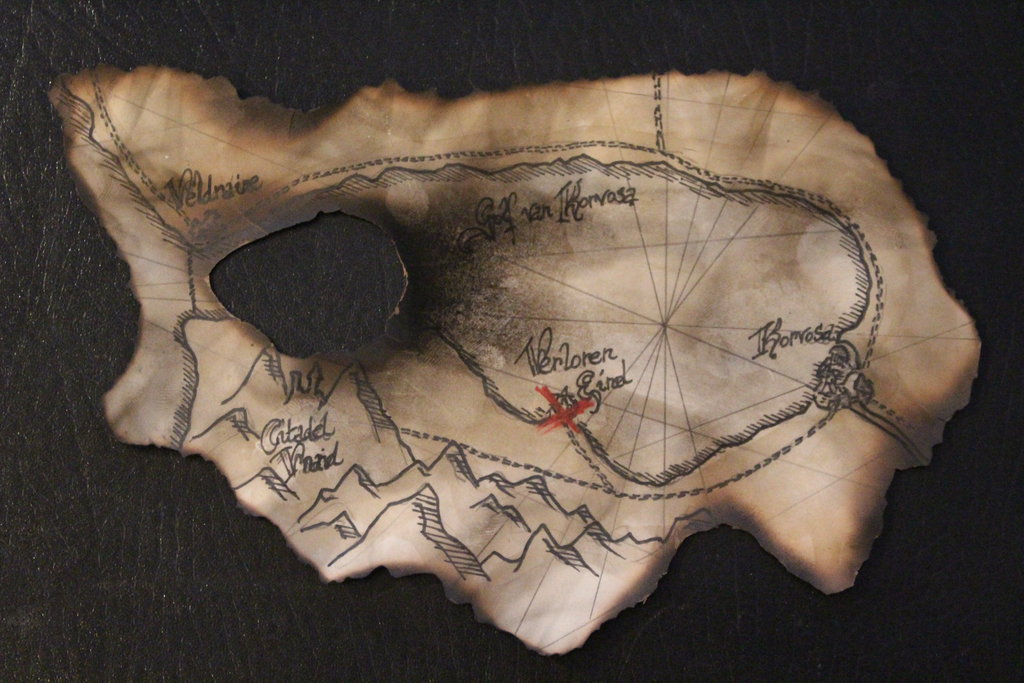
\includegraphics[width=0.39\textwidth]{images/Burned-map-for-curse-of-the-Crimson-Throne-503803899.jpg}
	\caption{Burned map for curse of the Crimson Throne}
	\label{fig:Burned-map-for-curse-of-the-Crimson-Throne-503803899}
\end{figure}

